\chapter{Heart rate sensor}\label{ch:heartRate}
%**********************************************

%**********************************************
\section{Introduction} \label{sec:heartIntro}
%**********************************************
Circuits pertaining to signal conditioning, pulse signal and analogue output generation will be discussed. Conditioning is done via filtering and amplification; active filters provide high input and low output impedance, and a large Q-factor \cite{actpas}. A differential amplifier is suitable for amplification, as the gain is referenced against a customizable voltage \cite{opamp}. A Schmitt Trigger is well-suited for pulse generation, as it provides a noise margin \cite{schmitt}. PWM signals can be converted to analogue using filtering \cite{PWM}. \textbf{check template at end to make sure everything is included}

%**********************************************
\section{Design} \label{sec:heartDesign}
%**********************************************
\begin{figure}[h]
    \centering
    \vspace{-0.7cm}
    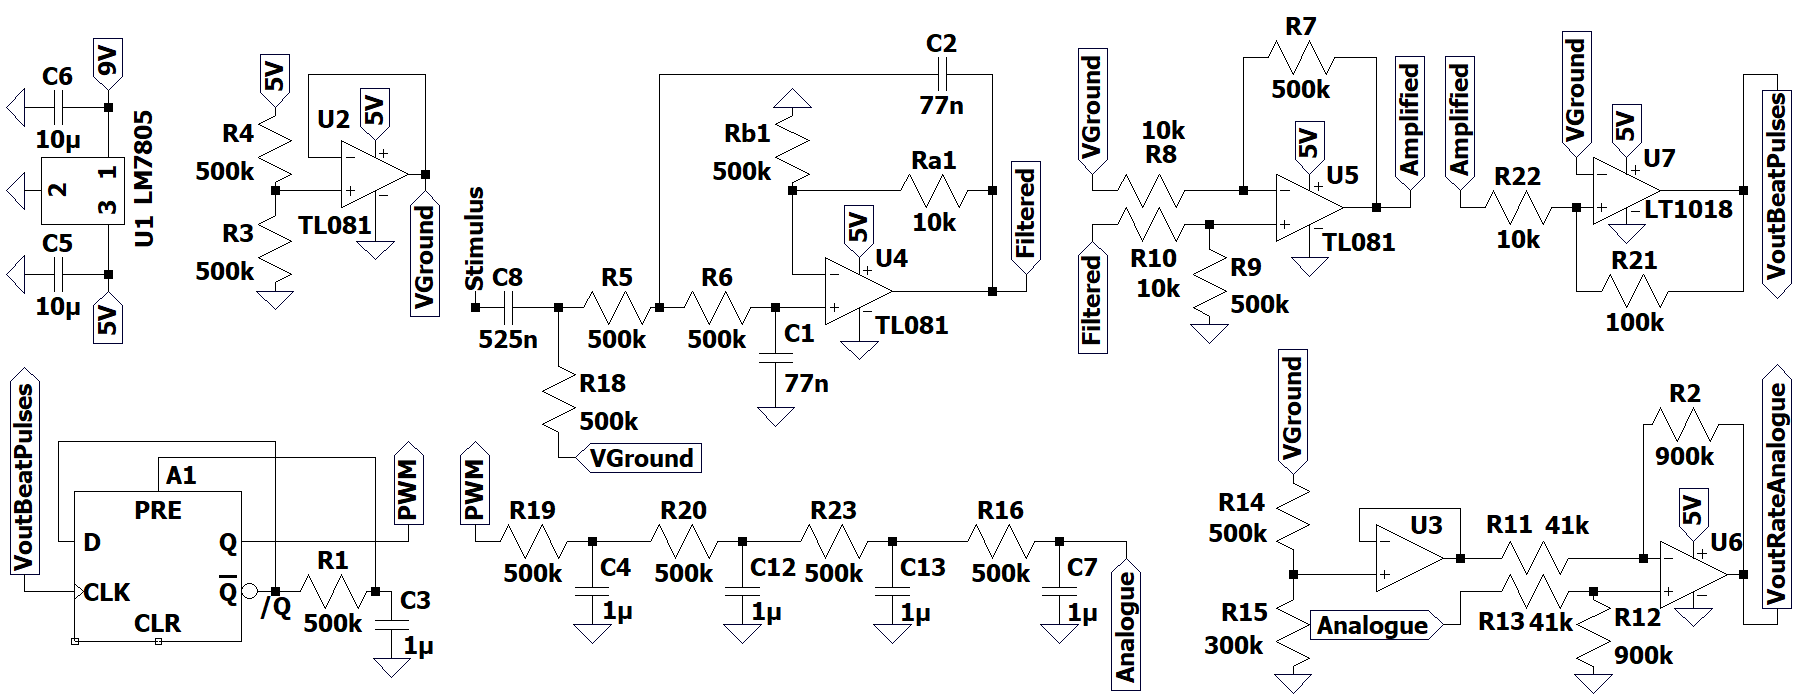
\includegraphics[width = 1\textwidth]{Figures/circuit}
    \caption{Complete Circuit \textbf{enlarge this}}
    \label{fig:circuit}
\end{figure}

The complete circuit is shown upfront in figure \ref{fig:circuit} in order to aid with explanation. Note that when resistor values are selected at random, the largest resistor in the sub-circuit is always chosen to be \SI{500}{k\Omega}, as to reduce current usage. The design process now follows.\\
The stimulus input signal contains noise at \SI{0.25}{Hz} and at \SI{5}{Hz} and higher. The information in the signal resides between \numrange{0.8}{2.5} \si{Hz}, corresponding to 50 and 150 BPM respectively. Noise results in distorted square wave output, necessitating filtering. A first order passive high-pass filter, cutoff frequency \SI{0.606}{Hz}, attenuates the low frequency noise. With R18 = \SI{500}{k\Omega}, C8 = \SI{525}{nF} according to $f_{c} = \frac{1}{2\pi R C}$. The capacitor is connected to a virtual ground of \SI{2.5}{V}, thus centering the signal around \SI{2.5}{V}. A second order active low-pass filter, cutoff frequency \SI{4.1}{Hz}, filters out high frequency noise. R5 = R6 = \SI{500}{k\Omega}, C1 = C2 = \SI{77}{nF} - see aforementioned formula. Cutoff frequencies were selected to remove noise maximally while minimally affecting heart-rate data. The signal should reside slightly above \SI{2.5}{V} to facilitate amplification (to be discussed). Thus, Rb1 = \SI{500}{k\Omega} and Ra1 = \SI{10}{k\Omega} since $A_v=1+\frac{R_{A}}{R_{B}}$ 
\cite{filter}. The TL081 op-amp is used, as it is less expensive than the TLC2272 \cite{octo}. A filter output with DC offset slightly above \SI{2.5}{V} allows for the use of a differential amplifier with the existing virtual ground connected to the negative input, thus removing the need for additional circuitry otherwise required to provide a voltage level at the negative input. The signal is amplified according to $\mathrm{V}_{\mathrm{OUT}}=\frac{\mathrm{R}_{a}}{\mathrm{R}_{b}}\left(\mathrm{V}_{2}-\mathrm{V}_{1}\right)$ \cite{opamp}, where R\textsubscript{a} corresponds to R7 and R9, and R\textsubscript{b} to R8 and R10. The gain of 50 was selected to again provide a DC offset of \SI{2.5}{V}, as it facilitates implementation of the comparator (to be discussed). Since the amplified signal has an amplitude of only \SI{1.66}{V}, the inexpensive TL081 was chosen despite having a smaller output range. Next, the signal is fed into a Schmitt Trigger comparator, which produces \SI{5}{V} if the input exceeds the upper trip point (UTP) and \SI{0}{V} if the input falls below the lower trip point (LTP) \cite{schmitt}. The range between the UTP and LTP is referred to as the hysteresis width and serves as a noise margin \cite{schmitt} around the reference voltage, $V_{REF}$. The hysteresis width was chosen as \SI{0.5}{V} as to be an order of magnitude larger than the highest levels of noise present on the signal serving as input to the comparator. As mentioned previously, the amplified signal has a DC offset of \SI{2.5}{V}, which was chosen as to require V\textsubscript{REF} = \SI{2.5}{V}, once again allowing for the use of the existing virtual ground (instead of additional circuitry) at the negative input of the LT1018 comparator. UTP = \SI{2.75}{V}, LTP = \SI{2.25}{V}, UTP = $V_{REF} + \beta Vcc$ and LTP = $V_{REF} - \beta Vcc$, thus $\beta$ = 0.05 \cite{schmitt}. Further, $\beta=\frac{\mathrm{R}_{22}}{\mathrm{R}_{22}+\mathrm{R}_{21}}$. Thus R21 = \SI{190}{k\Omega} and R22 = \SI{10}{k\Omega}. (R21 was later adjusted to \SI{100}{k\Omega} to account for loading effects). The design specifications require a pulse width of at least \SI{150}{ms}. A one-shot was considered to extend the pulses, but was omitted as the requirement could be met without it. All of the aforementioned thus produces a square wave output, where the frequency of the pulses directly relates to the heart-rate. \\\\\\\\

Obtaining an output suitable for a microcontroller presents itself as a problem of converting frequency to analogue. The decision was made to obtain a PWM signal from the FM pulse signal, as PWM signals lend themselves more readily to conversion-to-analogue using a simple low-pass RC filter. Pulse-width modulation was achieved by means of a D flip-flop. The essence of the design is to firstly keep the output high continually, but to then drive the output low for a fixed time, once per period. Since the period of the clock signal varies against BPM, driving low for a fixed amount of time results in a different ratio of the pulse being low at different frequencies, producing a varying duty cycle.

Specifically, the previously generated pulse signal is used as a clock signal for the D flip-flop, and the not-Q output is fed back into the data line. This would normally drive the output high for all time $t$; thus a RC circuit is added of which the capacitor is charged by the not-Q output, and connected to the SET-line of the flip-flop. Once the capacitor charges to \SI{2.5}{V}, Q is pulled high and not-Q low until the next rising edge of the clock input inverts Q and not-Q. The result is a slightly delayed PWM signal, with a large duty cycle at high frequencies, and vice-versa. This configuration was preferred above the standard one-shot setup, as it results in a linear and consistent PWM output, as long as the capacitor charge time is selected to be shorter than the narrowest pulse of the clock signal. The calculations follow\\

Select R1 = \SI{500}{k\Omega}. The capacitor charge oscillates between $V_L$ and $V_H$. $V_H =$ \SI{2.5}{V}. $V_L$ is reached for the first time at $t_{L_1}$ and $V_H$ at $t_{H_1}$. $V_L$ is then reached at  $t_{L_2}$. This gives:


$$V_L = 5\left(1-e^{\frac{t_{L_1}}{tau}}\right)$$
$$V_H = 5\left(1-e^{\frac{-t_H_1}{\tau}}\right)$$
$$V_L = V_H\left(e^{\frac{t_{L_1}}{tau}}\right)$$

See section \ref{sec:heartResults}, figure \ref{fig:pwm} for output graphs. 

Having obtained a PWM signal, filtering and amplification produce 

















\begin{figure}
 \footnotesize
   \centering
   \begin{subfigure}[]{0.45\textwidth}
        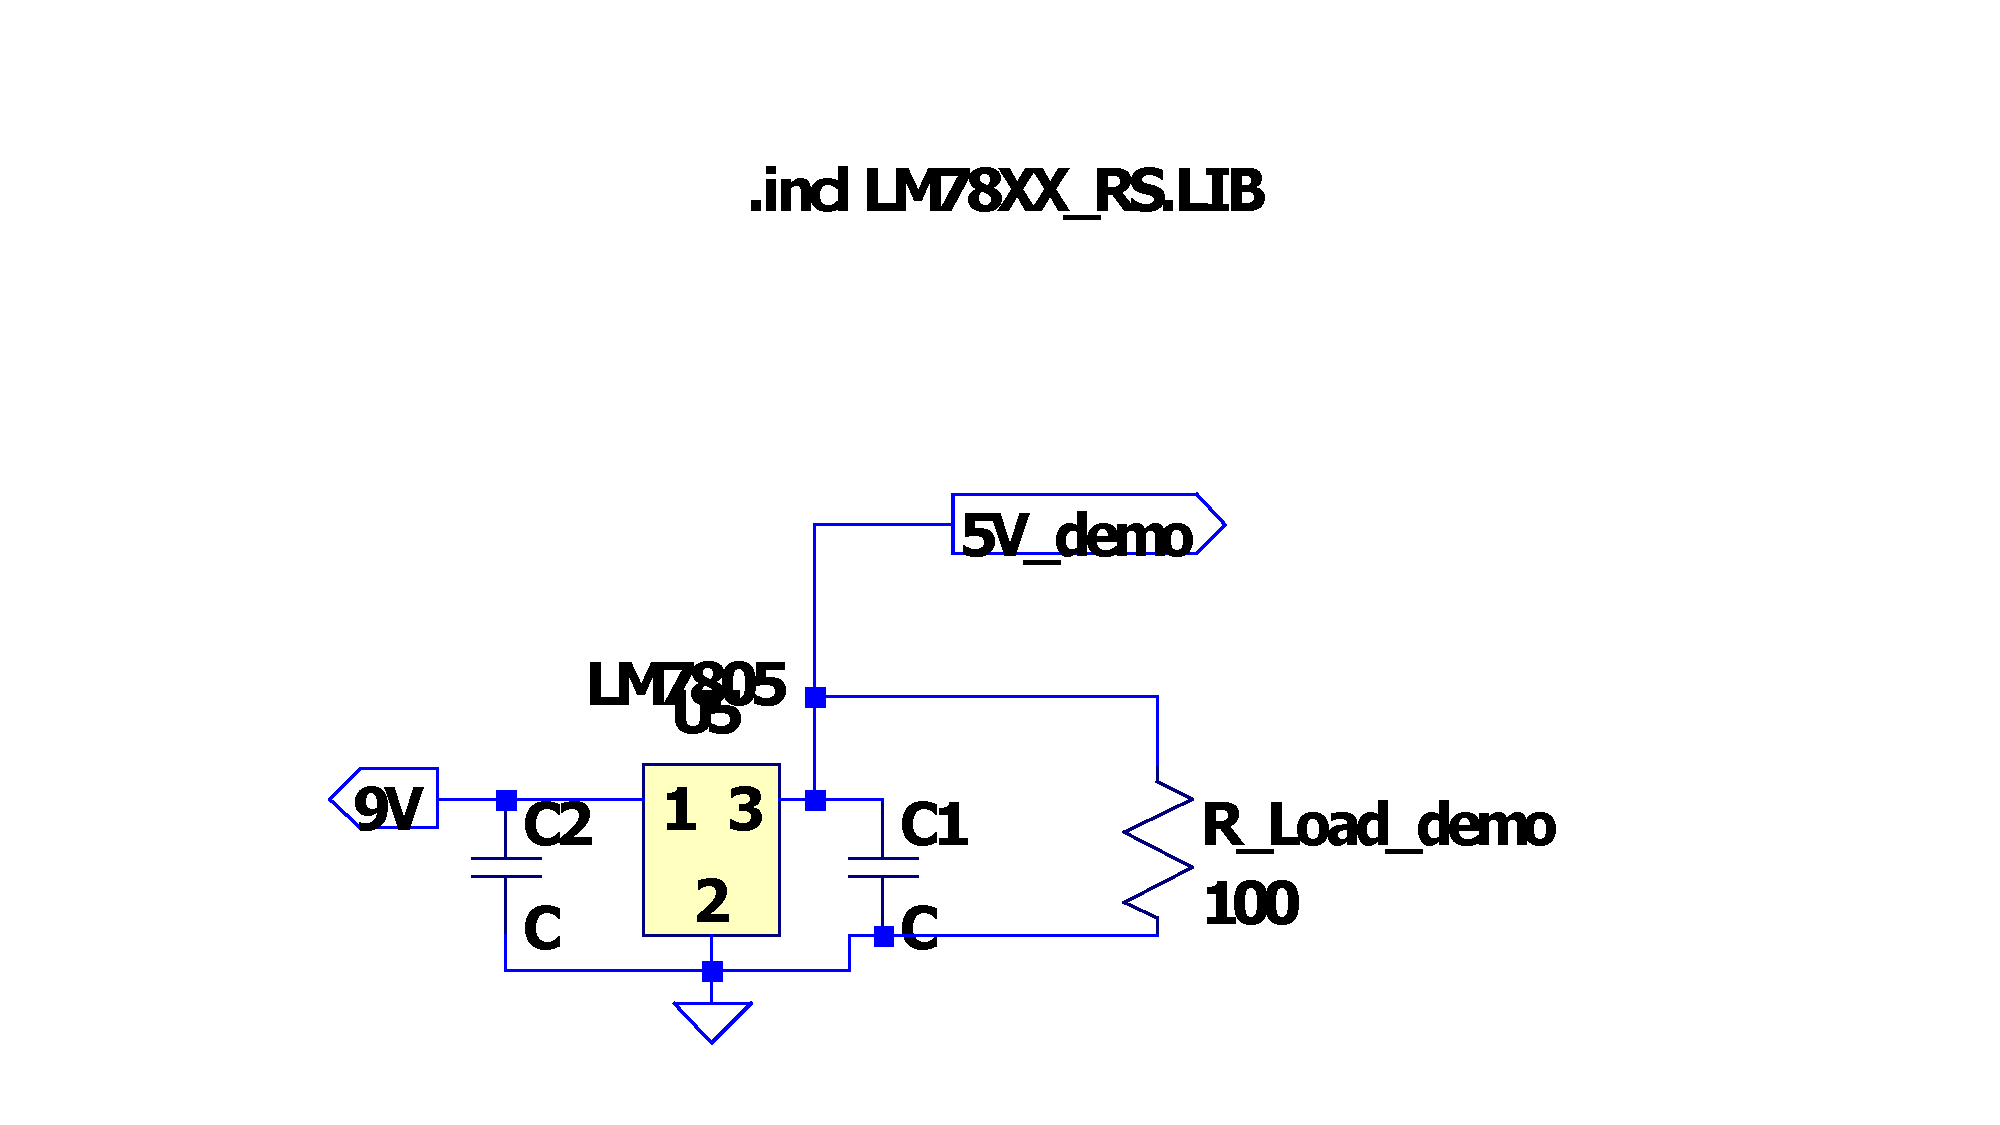
\includegraphics[width=\linewidth]{./Figures/E344_Ass1VoltRegulator_cct}
	  \caption{Linear voltage regulator.} \label{subfig:linear_circuit_diagram}	
   \end{subfigure}
   \begin{subfigure}[]{0.45\textwidth}
  	 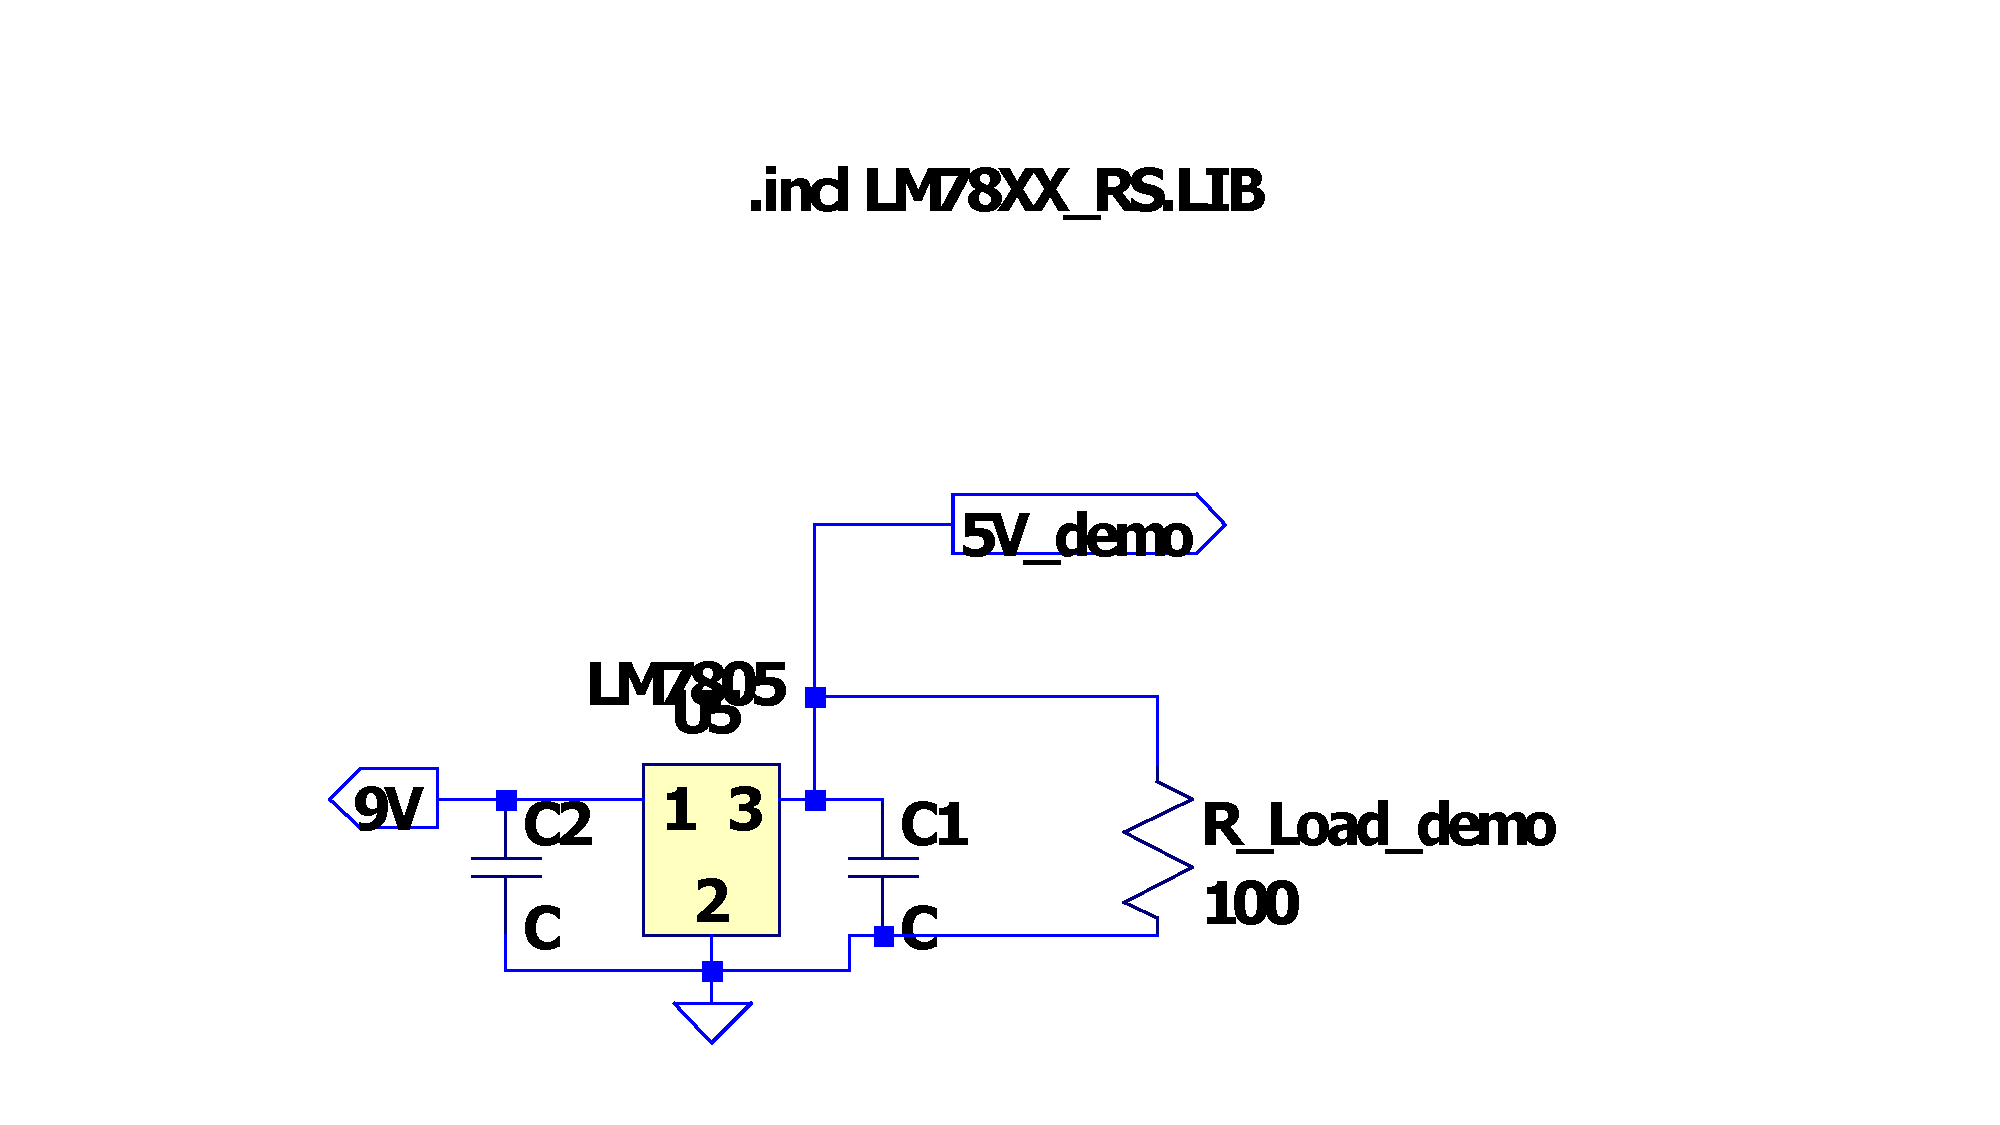
\includegraphics[width=\linewidth]{./Figures/E344_Ass1VoltRegulator_cct}
	  \caption{Switchmode voltage regulator.} \label{subfig:switchmode_circuit_diagram}	
   \end{subfigure}
   \begin{subfigure}[]{0.95\textwidth}
  	 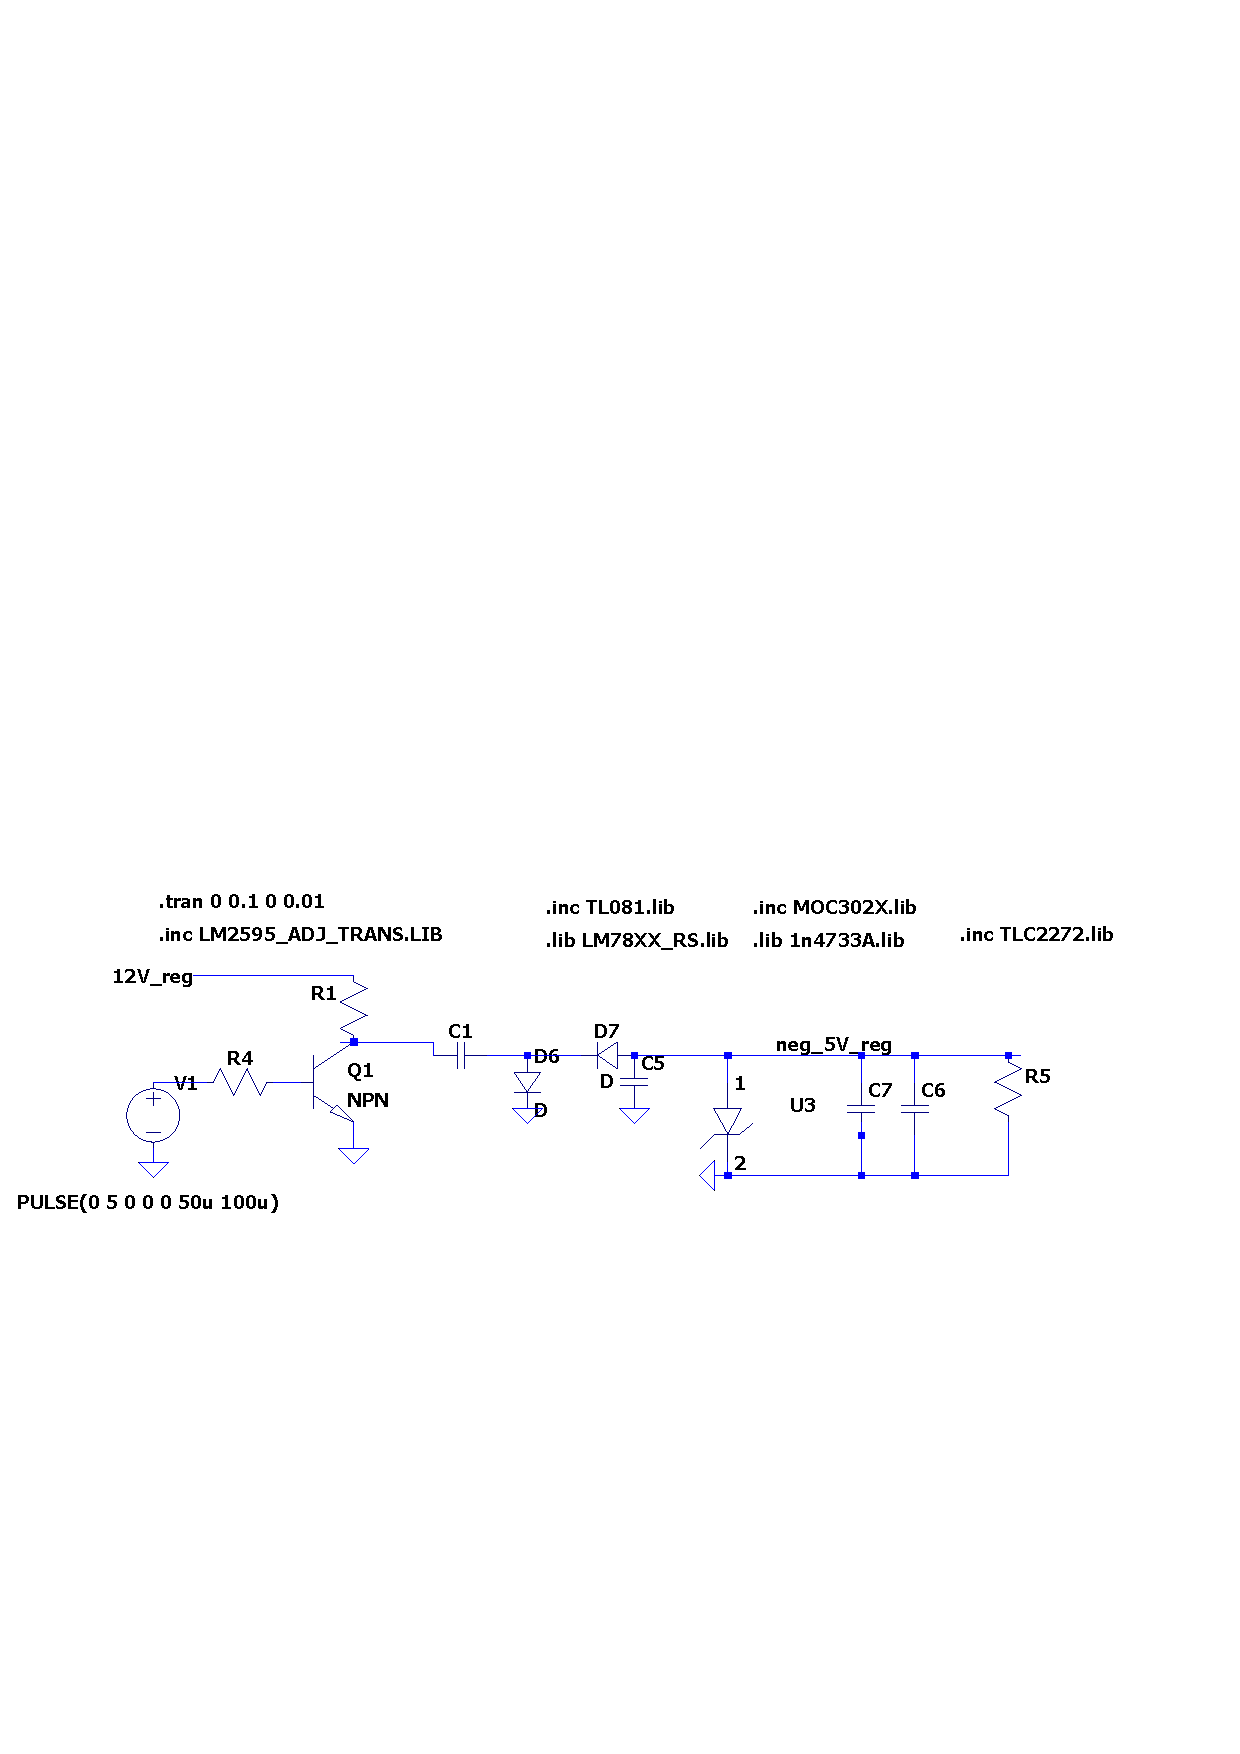
\includegraphics[width=\linewidth]{./Figures/CctDia}
	  \caption{Chargepump voltage regulator.} \label{subfig:chargepump_circuit_diagram}	
   \end{subfigure}
   
   \caption {Circuit diagrams of the two voltage regulators, and another irrelevant one}.

      \label{fig:circuit_diagram}
 \end{figure}
%**********************************************
\section{Results} \label{sec:heartResults}
%**********************************************


\begin{figure}
 \footnotesize
 \centering
    \begin{subfigure}[]{0.55\textwidth}
              \centering
  		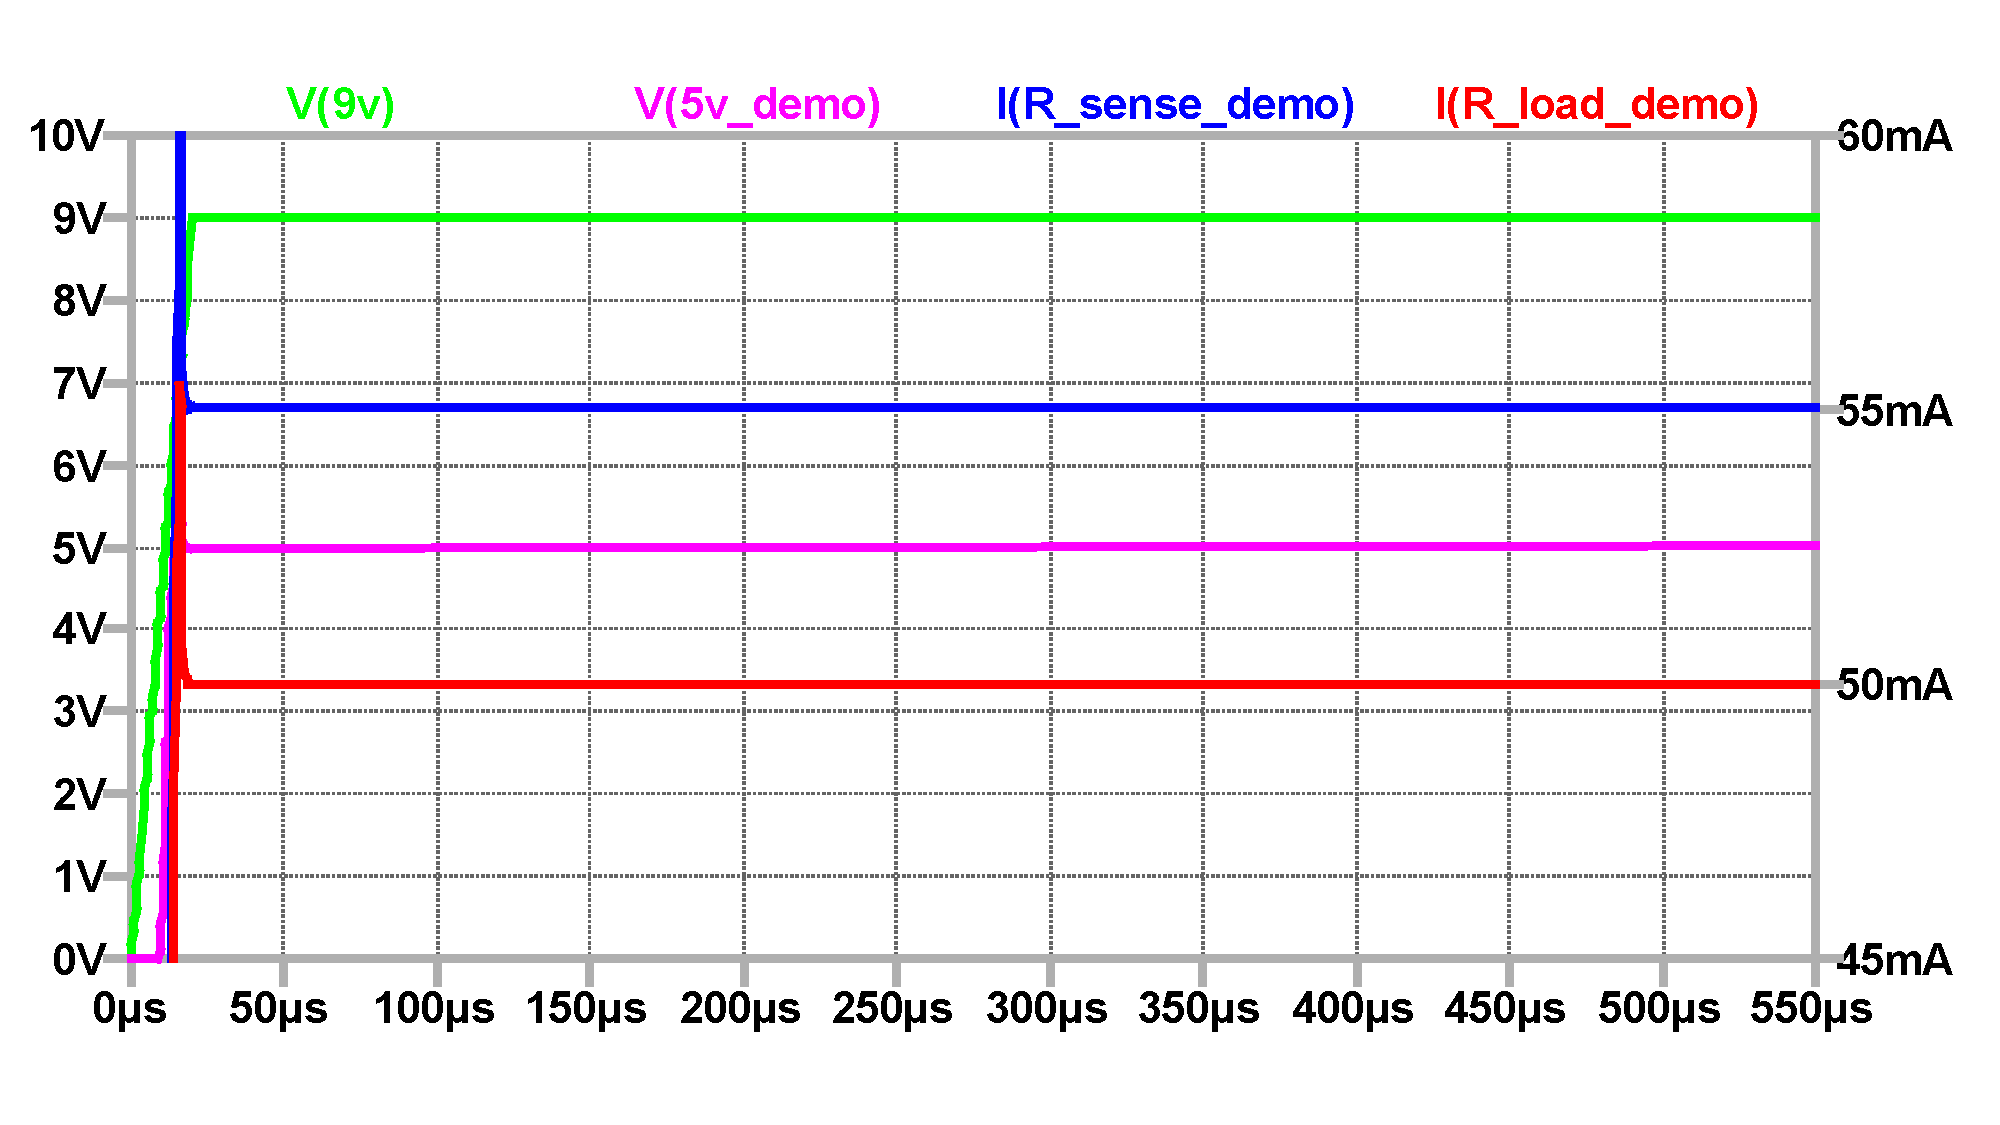
\includegraphics[width=1\linewidth]{./Figures/E344_VoltRegulator.pdf}
		    \caption{} \label{subfig:pwr_simu_rect}
     \end{subfigure}
     \begin{subfigure}[]{0.4\textwidth}
             \centering
  		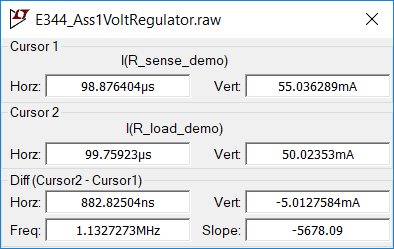
\includegraphics[width=1.0\linewidth]{./Figures/Screengrab2}
		   \caption{ } \label{subfig:pwr_meas_rect}
     \end{subfigure}
    \begin{subfigure}[]{0.55\textwidth}
              \centering
  		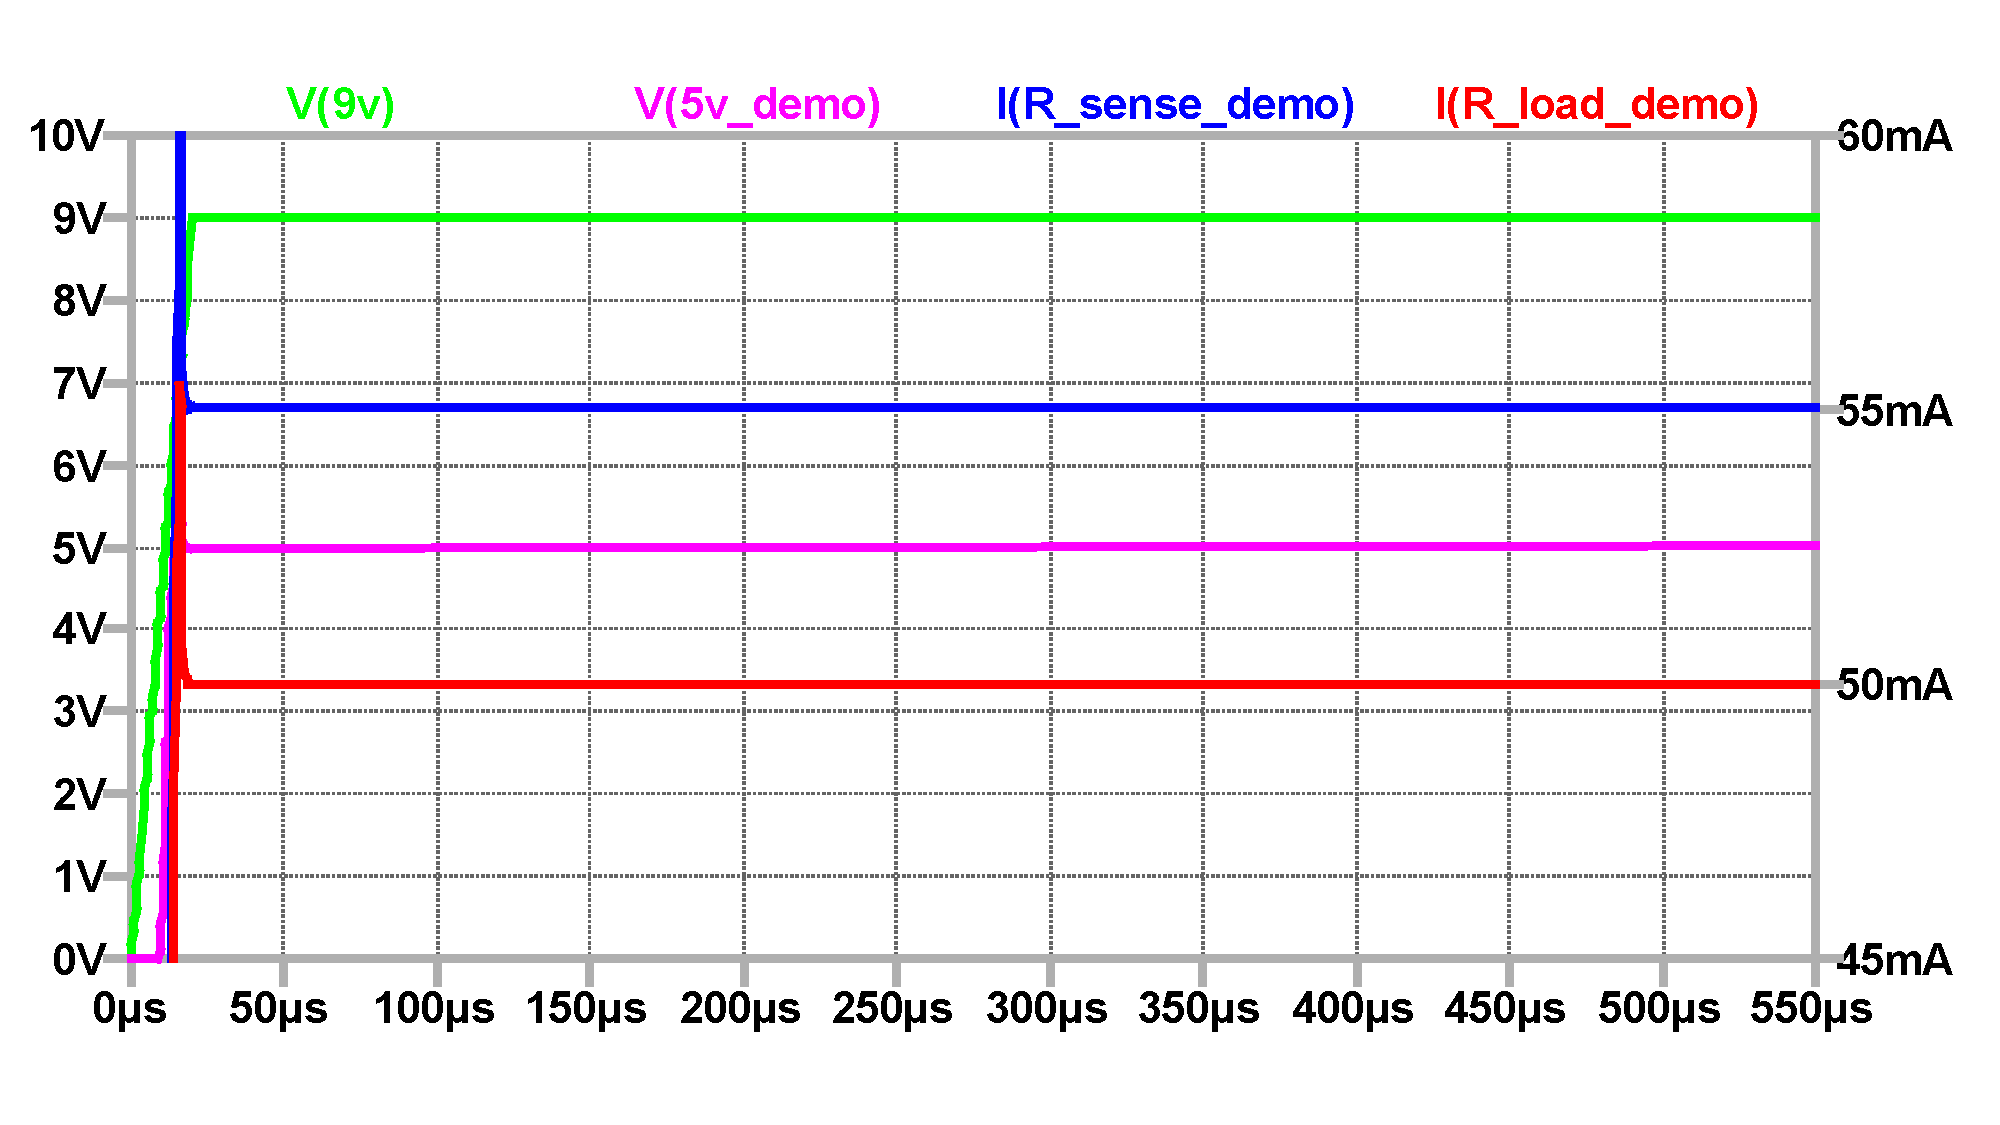
\includegraphics[width=1\linewidth]{./Figures/E344_VoltRegulator.pdf}
		    \caption{} \label{subfig:pwr_simu_rect}
     \end{subfigure}
    \begin{subfigure}[]{0.4\textwidth}
              \centering
  		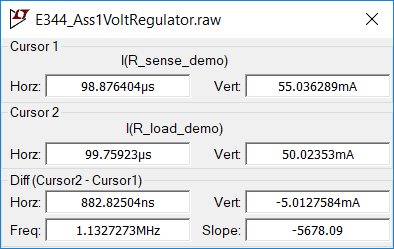
\includegraphics[width=1\linewidth]{./Figures/Screengrab2}
		    \caption{} \label{subfig:pwr_simu_rect}
     \end{subfigure}
   \caption[\textcolor{red}{I am the short caption that appears in the List of Figures list}]{Voltage regulation, comparing the linear and switchmode regulators... (a)  Blah blah. (b)  Blah blah.  (c)  Blah blah. (d) Blah blah.   As far as possible, please put input(s) and output(s) on the same plot rather than on separate plots. Based on the datasheet of XXXX in \cite{WebsiteOpAmp}}
    \label{fig:simulation_results_box}
 \end{figure}

In this section, you want to demonstrate, by means of referring to simulation results, using the designed circuit, how your circuit behaves as you designed it in Section \ref{sec:heartDesign}. Present and report on your simulated results in Figure \ref{fig:simulation_results_box}. Be absolutely sure that the text and information in your report are readable. 

You can use screengrabs or photos of the oscilloscope, or download the CSVs and plot them as PDFs using Matlab, Excel or similar. 
You can also use tables, example of which are presented in Tables \ref{tab:table1} and \ref{tab:table2}.


\begin{table}
        \centering
        \footnotesize
        \caption{Example of a simple table.}
         \begin{tabular}{c@{\qquad}rrrr}
          \toprule
             & 2017 & 2018 & $\Delta_{Abs}$ & $\Delta_{DiD}$\\
          \midrule
          A & 9,868      & 10,399 & +5 & -11\\
          B & 10,191     & 10,590 & +4 & -12\\
          \bottomrule
        \end{tabular}
     \label{tab:table1}
\end{table}


\begin{table}
         \centering
        \footnotesize
        \caption{Example of another table.}

         \begin{tabular}{c@{\qquad}rrrr}
          \toprule
          \multirow{2}{*}{\raisebox{-\heavyrulewidth}{Schools }} & \multicolumn{2}{c}{Total energy used}& \multicolumn{2}{c}{Change}\\
          \cmidrule{2-5}
            & 2017 & 2018 & $\Delta_{Abs}$ & $\Delta_{DiD}$\\
            & [kWh] & [kWh] & [\%] & [\%] \\
          \midrule
          A & 9,868      & 10,399 & +5 & -11\\
          B & 10,191     & 10,590 & +4 & -12\\
          \bottomrule
        \end{tabular}
     \label{tab:table2}
\end{table}


%**********************************************
\section{Summary}\label{sec:temp_summary}
%**********************************************
State whether your design performs as expected and what the limitations are or things to keep in mind are. 


